\section*{Learning Objectives}

\begin{itemize}
\item How to partition matrices into rows and columns
\item How to multiply two matrices
\item How to swap rows of a matrix
\end{itemize}

\section*{Outcomes}
\begin{itemize}
\item Multiplying a row vector by a column vector.
\item Recognizing the rows and columns of a matrix
\item Standard definition of matrix multiplication $A \cdot B$ using the rows of $A$ and the columns of $B$
   \item Size restrictions when multiplying matrices
\item Examples that work and those that don't because the sizes are wrong
    \item Introduce a second way of computing the product of two matrices using the columns of $A$ and the rows of $B$. This will later be used to compute the LU decomposition in a very simple way. 
    \item Permutation matrices
\end{itemize}

\newpage


\section{Multiplying a Row Vector by a Column Vector}

\begin{tcolorbox}[title=\textbf{The summation symbol}]

If you have not used it before, then the best way to learn it is via examples.
\begin{itemize}
    \item $1 + 2= \sum_{k=1}^{2} k $.  Here, $k$ is called an index and $\sum$ is the symbol for \textbf{sum or summation}. $\sum_{k=1}$ gives the initial value of the index in the sum, which in this case is 1, and  $\sum^2$ gives the final value of the index in the sum, which in this case, is 2.
    \item $1 + 2 + 3= \sum_{k=1}^{3} k $
    \item $1 + 2 + \cdots + n = \sum_{k=1}^{n} k $. We note that $\sum_{k=1}$ defines the initial value of the index in the sum to be 1, and  $\sum^n$ defines the final value of the index in the sum to be $n$.
    \item Changing the name of the index from $k$ to $i$, for example, does not change anything
    $$ \sum_{i=1}^{n} i =  1 + 2 + \cdots + n = \sum_{k=1}^{n} k $$
    \item $a_1+a_2 +a_3 =  \sum_{i=1}^{3} a_i$
    \item $a_7+a_8 +a_9 =  \sum_{i=7}^{9} a_i$. We note that the index is $i$, the initial value of the index is 7, and final value of the index is 9.
        \item $a_1+a_2 + \cdots + a_n =  \sum_{i=1}^{n} a_i$
    
\end{itemize}

\end{tcolorbox} 


Let $a^{\rm row}=\begin{bmatrix} a_1 & a_2 & \cdots & a_k \end{bmatrix}$ be a row vector with $k$ elements and let $b^{\rm col}= \begin{bmatrix} b_1 \\b_2 \\ \vdots \\b_k \end{bmatrix}$ be a column vector with the same number of elements as $a^{\rm row}$. The \textbf{product} of $a^{\rm row}$ and $b^{\rm col}$ is defined\footnote{If you have not seen the ``summation'' symbol before, here are some examples: $\sum_{i=1}^3 i:= 1 + 2 + 3$, $\sum_{i=5}^8 i:= 5 + 6 + 7 + 8$, and $\sum_{k=1}^n k^2:= 1 + (2)^2 + (3)^2 + \cdots + (n)^2.$} as 
\begin{equation}
\label{eq:VectorProductFormula}
    a^{\rm row} \cdot b^{\rm col}:= \sum_{i=1}^k a_i b_i := a_1 b_1 + a_2 b_2 + \cdots + a_k b_k.
\end{equation}
For many, the following visual representation is more understandable,
\begin{equation}
\label{eq:VectorProductVisual}
   \begin{bmatrix} a_1 & a_2 & \cdots & a_k \end{bmatrix} \cdot \begin{bmatrix} b_1 \\b_2 \\ \vdots \\b_k \end{bmatrix}:= a_1 b_1 + a_2 b_2 + \cdots + a_k b_k.
\end{equation}

\begin{tcolorbox}[title=\textbf{Remarks on Multiplying a Row Vector Times a Column Vector}]

\begin{itemize}
    \item It is very important to observe that the two vectors MUST have the same number of elements for their product to be defined.
    \item While \eqref{eq:VectorProductFormula} and \eqref{eq:VectorProductVisual} are equivalent (meaning they represent the same mathematical information), the formula in \eqref{eq:VectorProductFormula} is more convenient when writing a program and the visual representation in \eqref{eq:VectorProductVisual} is more convenient for hand computations.
    \item At this point, a column vector ``times'' a  row vector is not defined. When we do make sense of it, it will not be equal to $\sum_{i=1}^k a_i b_i.$
\end{itemize}

\end{tcolorbox} 

\begin{example}
\label{ex:RowTImesColumn01} 
Let $a^{\rm row}=\begin{bmatrix} 1 & 2 & 3 \end{bmatrix}$ be a row vector with $k=3$ elements and let $b^{\rm col}= \begin{bmatrix}4 \\5 \\ 6 \end{bmatrix}$ be a column vector with $k=3$ elements. Perform their multiplication if it makes sense.
\end{example}

\textbf{Solution:}
Because they have the same number of elements, we can form their product and we compute 
$$a^{\rm row} \cdot b^{\rm col}:= \sum_{i=1}^3 a_i b_i = (1)(4) + (2)(5) + (3)(6) = 32, $$
or we can look at it in the form
$$\begin{bmatrix} 1 & 2 & 3 \end{bmatrix} \cdot   \begin{bmatrix}4 \\5 \\ 6 \end{bmatrix} = (1)(4) + (2)(5) + (3)(6) = 32.$$
\Qed

\begin{example}
\label{ex:RowTImesColumn02} 
Let $a^{\rm row}=\begin{bmatrix} 1 & 2 & 3 \end{bmatrix}$ be a row vector with $k=3$ elements and let $b^{\rm col}= \begin{bmatrix}4 \\5  \end{bmatrix}$ be a column vector with $k=2$ elements. Perform their multiplication if it makes sense.
\end{example}

\textbf{Solution:}
Because they do NOT have the same number of elements, we cannot form their product. 
$$a^{\rm row} \cdot b^{\rm col}:= \text{undefined},$$
or 
$$\begin{bmatrix} 1 & 2 & 3 \end{bmatrix} \cdot  \begin{bmatrix}4 \\5  \end{bmatrix} = \text{error!}$$
\Qed  

\begin{example}
\label{ex:RowTImesColumn03} 
Let $a^{\rm row}=\begin{bmatrix} 2 & -3 & -1 & 11\end{bmatrix}$ be a row vector with $k=4$ elements and let $b^{\rm col}= \left[\begin{array}{r}3 \\5 \\ -1 \\ -2 \end{array} \right]$ be a column vector with $k=4$ elements. Perform their multiplication if it makes sense.
\end{example}

\textbf{Solution:}
Because they have the same number of elements, we can form their product and we compute 
$$a^{\rm row} \cdot b^{\rm col}:= \sum_{i=1}^4 a_i b_i = (2)(3) + (-3)(5) + (-1)(-1) + (11)(-2) = -30, $$
or, equivalently, we write it like this 
$$\begin{bmatrix} 2 & -3 & -1 & 11\end{bmatrix}\cdot  \left[\begin{array}{r}3 \\5 \\ -1 \\ -2 \end{array} \right] = (2)(3) + (-3)(5) + (-1)(-1) + (11)(-2) = -30. $$
\Qed  


\section{Examples of Row and Column Partitions}
%\noindent \textbf{Examples:}
Let $A=\left[\begin{array}{ccc} 1 & 2 & 3\\
4 & 5 & 6 \end{array}\right]$ be a $2\times 3$ matrix. Then a \textbf{partition} of $A$ \textbf{into rows is} 
$$\left[\begin{array}{c} a_1^{\rm row}\\
a_2^{\rm row} \end{array}\right]  = \left[\begin{array}{c}\boxed{ 1 ~~ 2 ~~ 3} \medskip \\
\boxed{4 ~~ 5 ~ ~6 }\end{array}\right],~~~\text{that is,}~~~\begin{aligned}
    a_1^{\rm row}= & [1 ~~ 2 ~~ 3] \medskip \\
    a_2^{\rm row}= & [4 ~~ 5 ~ ~6].
\end{aligned}$$
We note that $a_1^{\rm row}$ and $a_2^{\rm row}$ are row vectors of size $1 \times 3$; they have the same number of entries as $A$ has columns. \\

\textbf{A partition of} $A=\left[\begin{array}{ccc} 1 & 2 & 3\\
4 & 5 & 6 \end{array}\right]$ \textbf{into columns is} 
$$\left[\begin{array}{ccc} a_1^{\rm col} & a_2^{\rm col} & a_3^{\rm col}\end{array}\right]  = \left[ \boxed{\begin{array}{c} 1 \\ 4\end{array} }~~~
\boxed{ \begin{array}{c} 2 \\ 5\end{array} }~~~
\boxed{ \begin{array}{c} 3 \\ 6\end{array} }\right],~~~\text{that is,}~~~a_1^{\rm col}=\left[\begin{array}{c} 1\\
4 \end{array}\right],~~a_2^{\rm col}=\left[\begin{array}{c} 2\\
5 \end{array}\right],~~~a_3^{\rm col}=\left[\begin{array}{c} 3\\
6 \end{array}\right]
$$
We note that $a_1^{\rm col}$, $a_2^{\rm col}$, and $a_3^{\rm col}$ are column vectors of size $2 \times 1$; they have the same number of entries as $A$ has rows. \\


\section{General Case of Partitions}
Let $A$ be an $n \times m$ matrix. We recall that $n$ is the number of rows in $A$, $m$ is the number of columns, and $a_{ij}$ is the notation for the $ij$ element of $A$, that is, its value on the $i$-th row and $j$-th column. \textbf{A partition of $A$ into rows} is $$
 \left[\begin{array}{cccc} a_{11}& a_{12}& \cdots & a_{1m} \\
 a_{21}& a_{22}& \cdots & a_{2m}  \\
 \vdots & \vdots&  \ddots & \vdots \\
 a_{n1}& a_{n2}& \cdots & a_{nm} 
 \end{array}\right] = 
\left[\begin{array}{c} a_1^{\rm row} \medskip\\
a_2^{\rm row} \\
\vdots \\
a_n^{\rm row}\end{array}\right]  = \left[\begin{array}{c}\boxed{a_{11}~~ a_{12}~~ \cdots~~ a_{1m}} \medskip \\
\boxed{a_{21}~~ a_{22}~~ \cdots~~ a_{2m}} \\
\vdots \\
\boxed{a_{n1}~~ a_{n2}~~ \cdots~~ a_{nm}}\end{array}\right].$$
That is, the $i$-th row is the $1 \times m$ row vector
$$a_i^{\rm row} =[a_{i1}~~ a_{i2}~~ \cdots~~ a_{im}], $$
where $i$ varies from $1$ to $n$.\\

\textbf{A partition of $A$ into columns is} 
$$ \left[\begin{array}{cccc} a_{11}& a_{12}& \cdots & a_{1m} \\
 a_{21}& a_{22}& \cdots & a_{2m}  \\
 \vdots & \vdots&  \ddots & \vdots \\
 a_{n1}& a_{n2}& \cdots & a_{nm} 
 \end{array}\right] =
\left[\begin{array}{cccc} a_1^{\rm col} & a_2^{\rm col} & \cdots & a_m^{\rm col}\end{array}\right]  = \left[ \boxed{\begin{array}{c} a_{11} \\ a_{21}\\ \vdots \\ a_{n1}\end{array} }~~~
\boxed{\begin{array}{c} a_{12} \\ a_{22}\\ \vdots \\ a_{n2}\end{array} }~~~\cdots~~~
\boxed{\begin{array}{c} a_{1m} \\ a_{2m}\\ \vdots \\ a_{nm}\end{array} }\right].
$$
That is, the $j$-th column is the $n \times 1$ column vector
$$a_j^{\rm col} =\left[ \begin{array}{c} a_{1j} \\ a_{2j}\\ \vdots \\ a_{nj}\end{array} \right], $$
where $j$ varies from $1$ to $m$.\\

% \section{Building a Matrix from Column Vectors or Row Vectors}

% To be done. Emphasize the size restrictions. Do examples. General case. 


\section{Standard Matrix Multiplication: It's All About Rows and Columns}
\label{sec:StandardMatrixMultiplication}

Let $A$ be an $n \times k$ matrix, meaning it has $n$ rows and $k$ columns, and let $B$ be a $k \times m$ matrix, so that it has $k$ rows and $m$ columns. When the number of columns of the first matrix $A$ equals the number of rows of the second matrix $B$, the \textbf{matrix product} of $A$ and $B$ is defined and results in an $n \times m$ matrix:
$$[n\times k~~\text{matrix}] \cdot [k \times m~~\text{matrix}] = [n \times m~~\text{matrix}].$$
The values of $n, m$, and $k$ can be any integers greater than or equal to one. In particular, they can all be different numbers.


\begin{tcolorbox}

\begin{itemize}
    \item $[4\times 2~~\text{matrix}] \cdot [2 \times 5~~\text{matrix}] = [4 \times 5~~\text{matrix}].$
        \item $[1\times 11~~\text{matrix}] \cdot [11 \times 1~~\text{matrix}] = [1 \times 1~~\text{matrix}],$ which in Julia is different than a scalar.
            \item $[4\times 4~~\text{matrix}] \cdot [4 \times 4~~\text{matrix}] = [4 \times 4~~\text{matrix}].$
                        \item $[4\times 3~~\text{matrix}] \cdot [4 \times 4~~\text{matrix}] = \textbf{undefined}.$
\end{itemize}
\end{tcolorbox}

\begin{tcolorbox}[sharp corners, colback=green!30, colframe=green!80!blue, title=\textbf{\large Matrix multiplication using rows of $A$ and columns of $B$}]
The standard way of doing \textbf{matrix multiplication} $A \cdot B$ involves multiplying the rows of $A$ with the columns of $B$. We do some small examples before giving the general formula. \textbf{We will observe that the order in which we multiply two matrices is very important: \textcolor{red}{in general, $\mathbf{A \cdot B \neq B \cdot A}$ even when $A$ and $B$ are square matrices of the same size.}}
\end{tcolorbox}

\vspace*{.2cm}

\begin{tcolorbox}[title=\textcolor{red}{\bf \Large Source of the Definition of Matrix Multiplication}]

Here is an optional video by Michael Penn explaining WHY matrix multiplication needs to work this way: \url{https://youtu.be/cc1ivDlZ71U}. 
    
\end{tcolorbox}

\subsection{Examples}

\begin{example}
\label{ex:MatrixMultiplication01} 
We consider a $2 \times 2$ matrix $A$ and a $2 \times 1$ matrix $B$,
where we partition $A$ by rows and $B$ by columns. We note that the number of columns of $A$ matches the number of rows of $B$ so their product $A\cdot B$ is supposed to be defined. Let's do it! 
\end{example}

\textbf{Solution:}
\begin{equation}
  A=\left[\begin{array}{cc} 1 & 2 \\
3 & 4  \end{array}\right]  =   \left[\begin{array}{c} a_1^{\rm row}\\
a_2^{\rm row} \end{array}\right]  = \left[\begin{array}{c}\boxed{ 1 ~~ 2} \medskip\\
\boxed{3 ~~ 4 }\end{array}\right] ~~
\text{and}~~
    B=\left[\begin{array}{c} 5  \\ 6
\end{array}\right] = \Big[ b^{\rm col}_1 \Big] = \left[~\boxed{\begin{array}{c} 5 \\ 6\end{array} }~ \right].
\end{equation}
The matrix product of $A$ and $B$ is
\begin{equation}
    A \cdot B= \left[\begin{array}{c} a_1^{\rm row}\\
a_2^{\rm row} \end{array}\right] \cdot \Big[ b^{\rm col}_1 \Big]:=\left[  \begin{array}{c}  a_1^{\rm row} \cdot b_1^{\rm col} \\  a_2^{\rm row} \cdot b_1^{\rm col} \end{array} \right]
    = \left[\begin{array}{c} 17 \\ 39\end{array} \right]
\end{equation}
because
\begin{align*}
    a_1^{\rm row} \cdot b_1^{\rm col} &= \left[\begin{array}{cc} 1 & 2\end{array}\right] \cdot \left[\begin{array}{c} 5  \\ 6
\end{array}\right] = 5 + 12 = 17 \\
    a_2^{\rm row} \cdot b_1^{\rm col} &= \left[\begin{array}{cc} 3 & 4\end{array}\right] \cdot \left[\begin{array}{c} 5  \\ 6
\end{array}\right] = 15 + 24 = 39.
\end{align*}

A more visual way to do the multiplication is like this,
\begin{equation}
    A \cdot B=  \left[\begin{array}{c}\boxed{ 1 ~~ 2} \medskip \\
\boxed{3 ~~ 4 }\end{array}\right] \cdot 
  \left[~\boxed{\begin{array}{c} 5 \\ 6\end{array} }~ \right]   =  \left[\begin{array}{c} (1)(5)+(2)(6) \\ (3)(5)+(4)(6)\end{array} \right] =\left[\begin{array}{c} 17 \\ 39\end{array} \right]
\end{equation}
\Qed

\begin{tcolorbox}[title=\textbf{Remarks}]
\begin{itemize}
    \item A $2 \times 2$ matrix times a $2 \times 1$ matrix yields a $2 \times 1$ matrix.
    \item Let's observe that the operations for computing the matrix product boil down to performing the products of row vectors and column vectors of equal lengths! This is a general fact, as we will see. 
    \item Let's also recall that we do not know how to form the product of a row vector with a column vector when their lengths are not equal.
    \item  The number elements in $a_\bullet^{\rm row}$ is equal to the number of columns of $A$, while the number of elements in $b_\bullet^{\rm col}$ is equal to the number of rows of $B$. This is why the number of columns of $A$ must equal the number of rows of $B$ for their matrix product $A \cdot B$ to be defined.
\end{itemize}

\end{tcolorbox}

\begin{example}
\label{ex:MatrixMultiplication02} 
 We reuse $A$ and $B$ above and ask if we can form the matrix product in the order $B \cdot A$.
\end{example}

\textbf{Solution:}
 We have that the first matrix $B$ is $2 \times 1$ and the second matrix $A$ is $2 \times 2$. The number of columns of the first matrix does not match the number of rows of the second matrix, and hence the product cannot be defined in this direction. \Qed\\

\begin{example}
\label{ex:MatrixMultiplication03} 
 We consider a $2 \times 2$ matrix $A$ and a $2 \times 2$ matrix $B$. We note that the number of columns of $A$ matches the number of rows of $B$ so their product $A\cdot B$ is defined. We also note that the number columns of $B$ matches the number of rows of $A$, so the product $B \cdot A$ is also defined. This is a general property of square matrices $A$ and $B$ of the same size: their matrix product can be performed in either order. \textbf{We will note, however, that $\mathbf{A \cdot B \neq B \cdot A}$. Hence, when multiplying matrices, the order matters! }
\end{example}

\textbf{Solution:} 

\begin{equation}
\label{eq:Example3}
  A=\left[\begin{array}{cc} 1 & 2 \\
3 & 4  \end{array}\right]  =   \left[\begin{array}{c} a_1^{\rm row} \medskip\\
a_2^{\rm row} \end{array}\right]  = \left[\begin{array}{c}\boxed{ 1 ~~ 2} \medskip \\
\boxed{3 ~~ 4 }\end{array}\right] ~~
\text{and}~~
    B=\left[\begin{array}{cr} 5 & -2 \\ 6 & 1
\end{array}\right] = \Big[ b^{\rm col}_1 ~~  b^{\rm col}_2\Big] = \left[~\boxed{\begin{array}{c} 5 \\ 6\end{array} }~~\boxed{\begin{array}{r} -2 \\ 1\end{array} }~ \right].
\end{equation}
The matrix product of $A$ and $B$ is
\begin{equation}
   A \cdot B= \left[\begin{array}{c}\boxed{ 1 ~~ 2} \medskip \\
\boxed{3 ~~ 4 }\end{array}\right]  \cdot \left[~\boxed{\begin{array}{c} 5 \\ 6\end{array} }~~\boxed{\begin{array}{r} -2 \\ 1\end{array} }~ \right] =\left[\begin{array}{cc} (1)(5)+(2)(6) & (1)(-2)+(2)(1) \medskip \\
(3)(5)+(4)(6) & (3)(-2)+(4)(1)  \end{array}\right]  =\left[\begin{array}{rr} 17 & 0 \\
39 & -2  \end{array}\right].
\end{equation}
The matrix product of $B$ and $A$ is
\begin{equation}
\label{eq:BAexample}
   B \cdot A= \left[\begin{array}{c}\boxed{ 5 ~-2} \medskip\\
\boxed{6 ~~~~~ 1 }\end{array}\right]  \cdot \left[~\boxed{\begin{array}{c} 1 \\ 3\end{array} }~~\boxed{\begin{array}{r} 2 \\ 4\end{array} }~ \right] =\left[\begin{array}{cc} (5)(1)+(-2)(3) & (5)(2)+(-2)(4) \medskip \\
(6)(1)+(1)(3) & (6)(2)+(1)(4)  \end{array}\right]  =\left[\begin{array}{rr} -1 & 2 \\
9 & 16  \end{array}\right].
\end{equation}

\Qed

\begin{tcolorbox}[sharp corners, colback=green!30, colframe=green!80!blue, title=\textbf{\Large Order Matters When Multiplying Matrices}]

\begin{itemize}
    \item We note that $\left[\begin{array}{rr} 17 & 0 \\
39 & -2  \end{array}\right]= A \cdot B \neq B \cdot A = \left[\begin{array}{rr} -1 & 2 \\
9 & 16  \end{array}\right]$. The order in which matrices are multiplied matters. This is very different from the order of two real numbers, such as $\pi$ and $\sqrt{2}$, which you can multiply in either order and you always get the same answer!
    \item $A\cdot B:= \left[\begin{array}{cc} a_1^{\rm row} \cdot b_1^{\rm col} & a_1^{\rm row}\cdot  b_2^{\rm col}  \medskip \\
    a_2^{\rm row} \cdot b_1^{\rm col} & a_2^{\rm row} \cdot b_2^{\rm col}
\end{array}\right],$  where you can find $a_i^{\rm row} $ and $ b_j^{\rm col}$ highlighted in \eqref{eq:Example3}.
    \item $B\cdot A:= \left[\begin{array}{cc}  b_1^{\rm row}  \cdot a_1^{\rm col} & b_1^{\rm row}  \cdot a_2^{\rm col}  \medskip \\
    b_2^{\rm row}  \cdot a_1^{\rm col} & b_2^{\rm row}  \cdot a_2^{\rm col}
\end{array}\right],$ where you can find $b_i^{\rm row} $ and $ a_j^{\rm col}$ highlighted in \eqref{eq:BAexample}.
\end{itemize}

\end{tcolorbox}

\begin{example}
\label{ex:MatrixMultiplication04} 
For the given $3 \times 2$ matrix $A$ and $2 \times 2$ matrix $B$, compute $A \cdot B$ and $B \cdot A$ if the given multiplications make sense. 
$$A=\left[\begin{array}{cc} 1 & 2\\
3 & 4 \\ 5 & 6 \end{array}\right] \text{ and } B=\left[\begin{array}{ccc}
 3 &4  \\
2 & 1 \end{array}\right].$$
\end{example}

\textbf{Solution:}
We note that the number of columns of $A$ equals the number of rows of $B$ so their product $A\cdot B$ is defined. We also note that the number columns of $B$ does not equal the number of rows of $A$, so the product $B \cdot A$ is not defined.  
$$A=\left[\begin{array}{cc} 1 & 2\\
3 & 4 \\ 5 & 6 \end{array}\right] =  \left[\begin{array}{c} a_1^{\rm row} \medskip\\
a_2^{\rm row} \medskip \\ a_3^{\rm row} \end{array}\right]  = \left[\begin{array}{c}\boxed{ 1 ~~ 2} \medskip\\
\boxed{3 ~~ 4 } \medskip \\ \boxed{5 ~~ 6 }\end{array}\right]
~~\text{and}~~B=\left[\begin{array}{ccc}
 3 &4  \\
2 & 1 \end{array}\right] = \Big[ b^{\rm col}_1 ~~  b^{\rm col}_2\Big] = \left[~\boxed{\begin{array}{c} 3 \\ 2\end{array} }~~\boxed{\begin{array}{r} 4 \\ 1\end{array} }~ \right]$$
By now, you may have a favorite method, and using it, you should compute that
$$A \cdot B = \left[\begin{array}{cc} 7 & 6\\
17 & 16 \\ 27 & 26 \end{array}\right]$$ \Qed \\ 

\textbf{Remark:} When doing calculations by hand, $3 \times 3$ matrices are about as big as you ever really want to do. In Julia, ``the sky is the limit''. The following section is to help us understand what Julia is doing when it multiplies two matrices with the command \texttt{A * B}.

\subsection{Optional Read: General case: what is happening inside Julia}
We partition the $n \times k$ matrix $A$ into rows and the  $k \times m$ matrix $B$ into columns, as in 
\begin{equation}
   A= \left[\begin{array}{cccc} a_{11}& a_{12}& \cdots & a_{1k} \medskip \\
 a_{21}& a_{22}& \cdots & a_{2k}  \\
 \vdots & \vdots&  \ddots & \vdots \\
 a_{n1}& a_{n2}& \cdots & a_{nk} 
 \end{array}\right] = 
\left[\begin{array}{c} a_1^{\rm row}\\
a_2^{\rm row} \\
\vdots \\
a_n^{\rm row}\end{array}\right]  = \left[\begin{array}{c}\boxed{a_{11}~~ a_{12}~~ \cdots~~ a_{1k}}  \medskip \\
\boxed{a_{21}~~ a_{22}~~ \cdots~~ a_{2k}} \\
\vdots \\
\boxed{a_{n1}~~ a_{n2}~~ \cdots~~ a_{nk}}\end{array}\right]
\end{equation}
and
\begin{equation}
   B= \left[\begin{array}{cccc} b_{11}& b_{12}& \cdots & b_{1m} \\
 b_{21}& b_{22}& \cdots & b_{2m}  \\
 \vdots & \vdots&  \ddots & \vdots \\
 b_{k1}& b_{k2}& \cdots & b_{km} 
 \end{array}\right] =
\left[\begin{array}{cccc} b_1^{\rm col} & b_2^{\rm col} & \cdots & b_m^{\rm col}\end{array}\right]  = \left[ \boxed{\begin{array}{c} b_{11} \\ b_{21}\\ \vdots \\ b_{k1}\end{array} }~~~
\boxed{\begin{array}{c} b_{12} \\ b_{22}\\ \vdots \\ b_{k2}\end{array} }~~~\cdots~~~
\boxed{\begin{array}{c} b_{1m} \\ b_{2m}\\ \vdots \\ b_{km}\end{array} }\right],
\end{equation}
then
\begin{equation}
   A \cdot B:= 
\left[\begin{array}{cccc}  a_1^{\rm row} \cdot b_1^{\rm col} & a_1^{\rm row} \cdot b_2^{\rm col} & \cdots & a_1^{\rm row} \cdot b_m^{\rm col} \medskip  \\
a_2^{\rm row} \cdot b_1^{\rm col} & a_2^{\rm row} \cdot b_2^{\rm col} & \cdots & a_2^{\rm row} \cdot b_m^{\rm col} \\
\vdots & \vdots & \ddots & \vdots \\
a_n^{\rm row} \cdot b_1^{\rm col} & a_n^{\rm row} \cdot b_2^{\rm col} & \cdots & a_n^{\rm row} \cdot b_m^{\rm col}
\end{array}\right].
\end{equation}
Another way to see the pattern is like this
\begin{equation}
\label{eq:RowColumnMatrixMultiplication}
   A \cdot B:=  \left[\begin{array}{c}\boxed{a_{11}~~ a_{12}~~ \cdots~~ a_{1k}}  \medskip \\
\boxed{a_{21}~~ a_{22}~~ \cdots~~ a_{2k}} \\
\vdots \\
\boxed{a_{n1}~~ a_{n2}~~ \cdots~~ a_{nk}}\end{array}\right] \cdot 
\left[ \boxed{\begin{array}{c} b_{11} \\ b_{21}\\ \vdots \\ b_{k1}\end{array} }~~~
\boxed{\begin{array}{c} b_{12} \\ b_{22}\\ \vdots \\ b_{k2}\end{array} }~~~\cdots~~~
\boxed{\begin{array}{c} b_{1m} \\ b_{2m}\\ \vdots \\ b_{km}\end{array} }\right] =
%
\left[\begin{array}{cccc}  \sum\limits_{i=1}^k a_{1i}b_{i1} & \sum\limits_{i=1}^k a_{1i}b_{i2} & \cdots & \sum\limits_{i=1}^k a_{1i}b_{im}  \medskip \\
 \sum\limits_{i=1}^k a_{2i}b_{i1} & \sum\limits_{i=1}^k a_{2i}b_{i2} & \cdots & \sum\limits_{i=1}^k a_{2i}b_{im} \\
\vdots & \vdots & \ddots & \vdots \\
 \sum\limits_{i=1}^k a_{ni}b_{i1} & \sum\limits_{i=1}^k a_{ni}b_{i2} & \cdots & \sum\limits_{i=1}^k a_{ni}b_{im} \\
\end{array}\right].
\end{equation}

\begin{tcolorbox}[title=\textbf{Bottom Line on Standard Multiplication}] In the standard way of defining matrix multiplication, the
 $ij$-entry of $A \cdot B$ is obtained by multiplying the $i$-th row of $A$ by the $j$-th column of $B$ (whenever the multiplication makes sense, meaning that the number of columns of $A$ equals the number of rows of $B$). We will not use the following notation on a regular basis, but some of you may like it; if we let $[A \cdot B]_{ij}$ denote the $ij$-element of the matrix, $A\cdot B$, then 
 $$[A \cdot B]_{ij} := a_i^{\rm row} \cdot b_j^{\rm col}. $$
\end{tcolorbox}
 



\section{Multiplication by Summing over Columns and Rows}
\label{sec:NovelMatrixMultiplication}

\begin{tcolorbox}[sharp corners, colback=green!30, colframe=green!80!blue, title=\textbf{\large Rock your World: an Alternative Formula for Matrix Multiplication}]

\begin{itemize}
    \item We now introduce an alternative way to compute the product of two matrices. It gives the same answer as the ``standard method''.  \textbf{Very few people use or even know this definition because, for hand calculations, it takes more time to write out the individual steps.} ROB 101, however, is about computational linear algebra, and hence we ignore such trivial concerns as what is best for doing hand calculations! 
    
    \item We will see shortly that understanding this alternative way of matrix multiplication will allow us to solve almost any system of linear equations via a combination of forward and back substitution.

\item Instead of solving one hard system of linear equations, we will find the solution by solving two triangular systems of linear equations, one upper triangular and one lower triangular!
\end{itemize}
\end{tcolorbox}
\vspace*{.2cm}

 We reconsider two matrices $A$ and $B$ from Example~\ref{ex:MatrixMultiplication04}, but this time we partition $A$ into columns and $B$ into rows
 $$A=\left[\begin{array}{cc} 1 & 2\\
3 & 4 \\ 5 & 6 \end{array}\right] = \left[\begin{array}{cc} a_1^{\rm col} & a_2^{\rm col} \end{array}\right]  = 
\left[ \boxed{\begin{array}{c} 1 \\ 3 \\ 5\end{array} }~~~
\boxed{\begin{array}{c} 2 \\ 4 \\ 6\end{array} }\right]
~~\text{and}~~B=\left[\begin{array}{ccc}
 3 &4  \\
2 & 1 \end{array}\right] = \left[\begin{array}{c} b_1^{\rm row} \medskip \\
b_2^{\rm row} \end{array}\right]  = \left[\begin{array}{c}\boxed{ 3 ~~ 4} \medskip\\
\boxed{ 2 ~~ 1}
\end{array} \right].$$

What happens when we form the sum of the columns of $A$ times the rows of $B$,
$$a_1^{\rm col}  b_1^{\rm row} + a_2^{\rm col}  b_2^{\rm row} = \textbf{\Large ?}$$
We first observe that the columns of $A$ are $3 \times 1$ while the rows of $B$ are $1 \times 2$. Hence, their product with the usual rules of matrix multiplication will be $3 \times 2$, the same size as $A \cdot B$. That seems interesting. We do the two multiplications and obtain
$$
a_1^{\rm col} \cdot  b_1^{\rm row}= \left[\begin{array}{c} 1 \\
3 \\ 5 \end{array}\right] \cdot 
\left[\begin{array}{cc}3 & 4 \end{array}\right] =
\left[\begin{array}{cc} (1)\cdot (3) & (1)\cdot (4) \medskip\\
(3) \cdot (3) & (3) \cdot (4) \medskip \\ (5) \cdot (3) & (5) \cdot (4) \end{array}\right] =
\left[\begin{array}{cc} 3 & 4\\
9 & 12 \\ 15 & 20 \end{array}\right]$$
%
$$
a_2^{\rm col}  \cdot b_2^{\rm row}= 
\left[\begin{array}{c} 2 \\
4 \\ 6 \end{array}\right] \cdot 
\left[\begin{array}{cc}2 & 1 \end{array}\right] = 
\left[\begin{array}{cc} (2) \cdot (2) & (2) \cdot (1) \medskip\\
(4) \cdot (2) & (4) \cdot (1) \medskip \\ (6) \cdot (2) & (6) \cdot (1) \end{array}\right] =
\left[\begin{array}{cc} 4 & 2\\
8 & 4 \\ 12 & 6 \end{array}\right]$$
and hence their sum is
%
$$a_1^{\rm col}  b_1^{\rm row} + a_2^{\rm col}  b_2^{\rm row} = \left[\begin{array}{cc} 3 & 4\\
9 & 12 \\ 15 & 20 \end{array}\right] + \left[\begin{array}{cc} 4 & 2\\
8 & 4 \\ 12 & 6 \end{array}\right] = \left[\begin{array}{cc} 7 & 6\\
17 & 16 \\ 27 & 26 \end{array}\right]=A \cdot B$$

% \begin{verbatim}
%  A=[ 1 2; 3 4; 5 6]
%  B=[3 4; 2 1]
 
%  A(:,1)*B(1,:)
 
%  A(:,2)*B(2,:)

%      7     6
%     17    16
%     27    26
% \end{verbatim}

So while the bookkeeping is a bit different, the individual computations are easier than in the standard way of performing matrix multiplication, and perhaps they are also easier to get right. You're free to do your matrix multiplications as you wish. This particular method has a theoretical benefit that we will uncover shortly. Keep in mind that not so many people think of matrix multiplication as ``sums of columns times rows'' and you might confuse friends and other instructors when you talk about it in this manner. In fact, you may be told that you are wrong and that no one ever does it that way, even if it is correct. \\

%\vspace*{2cm}

\begin{tcolorbox}[sharp corners, colback=green!30, colframe=green!80!blue, title=\textbf{\large General Case of Matrix Multiplication using Columns of $\mathbf{A}$ and Rows of $\mathbf{B}$}]
 Suppose that $A$ is $n \times k$ and $B$ is $k \times m$ so that the two matrices are compatible for matrix multiplication. Then 
$$A\cdot B = \sum_{i=1}^{k} a_i^{\rm col} \cdot b_i^{\rm row},  $$
the ``sum of the columns of $A$ multiplied by the rows of $B$''. A more precise way to say it would be ``the sum over $i$ of the $i$-th column of $A$ times the $i$-th row of $B$.'' In HW, we'll play with this idea enough that it will become ingrained into your subconscious!
\end{tcolorbox}

\vspace*{.2cm}

\begin{tcolorbox}[title=\textbf{\large Alpha Go Takes on Matrix Multiplication}]
 Who would have guessed that there is still much innovation to be done in this space! You may enjoy these videos:

 \begin{itemize}
     \item \url{https://youtu.be/8ILk4Wjo5rc} AlphaTensor by DEEPMIND finds new Algorithms for Matrix Multiplication

     \item \url{https://youtu.be/CoFvu-n-fFs} AI Just Solved a 53-Year-Old Problem! | AlphaTensor, Explained
 \end{itemize}
\end{tcolorbox}


\section{(Optional Read:) Why the Second Method of Matrix Multiplication Works}

ROB 101 does not focus on proofs. Yet, sometimes it is genuinely fun to understand how or why things are as they are! We consider two $2 \times 2$ matrices $A$ and $B$, where
$$A= \left[\begin{array}{cc} a_{11}& a_{12} \\ a_{21} & a_{22}\end{array}\right]
\text{ and } B= \left[\begin{array}{cc} b_{11}& b_{12} \\ b_{21} & b_{22}\end{array}\right]
.$$
Then, using the standard rows of $A$ times the columns of $B$ formulation of matrix multiplication yields
$$
\begin{aligned}
 A \cdot B := &
\left[\begin{array}{cc}  a_1^{\rm row} \cdot b_1^{\rm col} & a_1^{\rm row} \cdot b_2^{\rm col}  \medskip  \\
a_2^{\rm row} \cdot b_1^{\rm col} & a_2^{\rm row} \cdot b_2^{\rm col}
\end{array}\right] \\ 
=& \left[\begin{array}{cc}  a_{11} b_{11} + a_{12}b_{21} & a_{11} b_{12} + a_{12}b_{22} \\
a_{21} b_{11} + a_{22}b_{21} & a_{21} b_{12} + a_{22}b_{22}
\end{array}\right]\bigskip  \text{(we take the sum outside the matrix)}\\
=& \left[\begin{array}{cc}  a_{11} b_{11}  & a_{11} b_{12} \\
a_{21} b_{11}  & a_{21} b_{12} 
\end{array}\right] + \left[\begin{array}{cc}  a_{12} b_{21}  & a_{12} b_{22} \\
a_{22} b_{21}  & a_{22} b_{22} 
\end{array}\right] \bigskip  \text{(we recognize each term)}\\
=& \left[\begin{array}{c} a_{11}\\ a_{21} \end{array}\right] \cdot 
 \left[\begin{array}{cc} b_{11}& b_{12} \end{array}\right] + 
 \left[\begin{array}{c} a_{12}\\ a_{22} \end{array}\right] \cdot 
 \left[\begin{array}{cc} b_{21}& b_{22} \end{array}\right]\\
=& a^{\rm col}_1 \cdot b^{\rm row}_1 + a^{\rm col}_2 \cdot b^{\rm row}_2
\end{aligned}
$$

In a similar manner, we can treat the general case. For those who wish to brave a blaze of indices, from \eqref{eq:RowColumnMatrixMultiplication}, we have
\begin{equation}
\begin{aligned}
   A \cdot B:=&  \left[\begin{array}{c}\boxed{a_{11}~~ a_{12}~~ \cdots~~ a_{1k}}  \medskip \\
\boxed{a_{21}~~ a_{22}~~ \cdots~~ a_{2k}} \\
\vdots \\
\boxed{a_{n1}~~ a_{n2}~~ \cdots~~ a_{nk}}\end{array}\right] \cdot 
\left[ \boxed{\begin{array}{c} b_{11} \\ b_{21}\\ \vdots \\ b_{k1}\end{array} }~~~
\boxed{\begin{array}{c} b_{12} \\ b_{22}\\ \vdots \\ b_{k2}\end{array} }~~~\cdots~~~
\boxed{\begin{array}{c} b_{1m} \\ b_{2m}\\ \vdots \\ b_{km}\end{array} }\right] \\
=&
%
\left[\begin{array}{cccc}  \sum\limits_{i=1}^k a_{1i}b_{i1} & \sum\limits_{i=1}^k a_{1i}b_{i2} & \cdots & \sum\limits_{i=1}^k a_{1i}b_{im}  \medskip \\
 \sum\limits_{i=1}^k a_{2i}b_{i1} & \sum\limits_{i=1}^k a_{2i}b_{i2} & \cdots & \sum\limits_{i=1}^k a_{2i}b_{im} \\
\vdots & \vdots & \ddots & \vdots \\
 \sum\limits_{i=1}^k a_{ni}b_{i1} & \sum\limits_{i=1}^k a_{ni}b_{i2} & \cdots & \sum\limits_{i=1}^k a_{ni}b_{im} \\
\end{array}\right] \text{ (we pull the sum outside the matrix)}\\
=& \sum\limits_{i=1}^k
\left[\begin{array}{cccc}   a_{1i}b_{i1} &a_{1i}b_{i2} & \cdots &  a_{1i}b_{im}  \medskip \\
     a_{2i}b_{i1} & a_{2i}b_{i2} & \cdots &  a_{2i}b_{im} \\
\vdots & \vdots & \ddots & \vdots \\
  a_{ni}b_{i1} & a_{ni}b_{i2} & \cdots &  a_{ni}b_{im} \\
\end{array}\right] \text{(we recognize what this is)}\\
=& \sum_{i=1}^{k} a_i^{\rm col} \cdot b_i^{\rm row} \\
=&
\left[ \boxed{\begin{array}{c} a_{11} \\ a_{21}\\ \vdots \\ a_{n1}\end{array} }~~~
\boxed{\begin{array}{c} a_{12} \\ a_{22}\\ \vdots \\ a_{n2}\end{array} }~~~\cdots~~~
\boxed{\begin{array}{c} a_{1k} \\ a_{2k}\\ \vdots \\ a_{nk}\end{array} }\right] \cdot  \left[\begin{array}{c}\boxed{b_{11}~~ b_{12}~~ \cdots~~ b_{1m}}  \medskip \\
\boxed{b_{21}~~ b_{22}~~ \cdots~~ b_{2m}} \\
\vdots \\
\boxed{b_{k1}~~ b_{k2}~~ \cdots~~ b_{km}}\end{array}\right]. \
\end{aligned}
\end{equation}

\section{Permutation Matrices: The Matrix View of Swapping the Order of Equations}
\label{sec:PermutationMatrices}

%\jwg{Uses matrix transpose before it is taught.}

Back in Sec.~\ref{sec:SwappingRows}, we made a brief remark on swapping rows of equations to put them into a nicer form. For simplicity, we recall the equations again here.\\

This system of equations is neither upper triangular nor lower triangular
\begin{equation}
\label{eq:BeforeSwapping}
    \begin{aligned}
     3 x_1 &=6 \\
    x_1 - 2 x_2 + 3 x_3  &= 2 \\
         2 x_1 - x_2 &= -2,
    \end{aligned}
\end{equation}
but if we simply re-arrange the order of the equations, we arrive at the lower triangular equations
\begin{equation}
\label{eq:AfterSwapping}
    \begin{aligned}
     3 x_1 &=6 \\
         2 x_1 - x_2 &= -2 \\
             x_1 - 2 x_2 + 3 x_3  &= 2.
    \end{aligned}
\end{equation}
As we noted before, we still have the same equations and hence their solution has not changed. The equations have just been re-arranged to make the process of computing their solution fall into a nice pattern that we already know how to handle.\\

We now write out the matrix equations for the ``unfortunately ordered'' equations ~\eqref{eq:BeforeSwapping} and then the ``nicely'' re-arranged system of equations \eqref{eq:AfterSwapping}
$$
 \underbrace{\left[\begin{array}{rrr} 3 & 0 & 0\\
1 & -2 & 3 \\ 2 & -1 & 0 \end{array}\right]}_{A_{O}}\underbrace{\left[\begin{array}{c} x_1 \\x_2 \\x_3\end{array} \right]}_{x}
= \underbrace{\left[\begin{array}{r} 6 \\2 \\-2\end{array} \right]}_{b_O} \hspace*{1cm}  \underbrace{\left[\begin{array}{rrr} 3 & 0 & 0\\
 2 & -1 & 0\\ 1 & -2 & 3 \\ \end{array}\right]}_{A_{L}}\underbrace{\left[\begin{array}{c} x_1 \\x_2 \\x_3\end{array} \right]}_{x}
= \underbrace{\left[\begin{array}{r} 6 \\-2 \\2\end{array} \right]}_{b_L}.$$
We see the second and third rows are swapped when we compare $A_O$ to $A_L$ and $b_O$ to $b_L$. 
The swapping of rows can be accomplished by multiplying $A_O$ and $b_O$ on the left by
$$ \mathbf{
P =\left[\begin{array}{rrr} 1 & 0 & 0\\
0 & 0 & 1 \\ 0 & 1 & 0 \end{array}\right]}.$$
Indeed, we check that
$$P \cdot A_O=\left[\begin{array}{rrr} 1 & 0 & 0\\
0 & 0 & 1 \\ 0 & 1 & 0 \end{array}\right] \left[\begin{array}{rrr} 3 & 0 & 0\\
1 & -2 & 3 \\ 2 & -1 & 0 \end{array}\right] = \left[\begin{array}{rrr} 3 & 0 & 0\\
 2 & -1 & 0\\ 1 & -2 & 3  \end{array}\right] = A_L $$
 and 
$$P \cdot b_O=\left[\begin{array}{rrr} 1 & 0 & 0\\
0 & 0 & 1 \\ 0 & 1 & 0 \end{array}\right]\left[\begin{array}{r} 6 \\2 \\-2\end{array} \right] = \left[\begin{array}{r} 6 \\-2 \\2\end{array} \right] = b_L. $$\
$\mathbf{P}$ \textbf{is called a permutation matrix}. \\

\begin{tcolorbox}[title=\textbf{Key Insight on Swapping Rows}] We note that the permutation matrix $P$ is constructed from the $3 \times 3$ identity matrix $I$ by swapping its second and third rows, exactly the rows we wanted to swap in $A_O$ and $b_O$. This observation works in general. 
\end{tcolorbox}

For example, suppose we want to do the following rearrangement
\begin{equation}
\label{eq:Permuation}
     \left[\begin{array}{r} 1 \\2 \\3 \\ 4 \\ 5\end{array} \right] \leftrightarrow \left[\begin{array}{r} 4 \\2 \\5 \\ 1 \\ 3\end{array} \right],
\end{equation}
where rows one and four are swapped and three and five are swapped. We have shown the arrow as going back and forth ($\leftrightarrow$) because applying the swap twice results in the original arrangement. To see the resulting structure at a matrix level, we put the $5 \times 5$ identity matrix on the left and the permutation matrix $P$ on the right
$$
I=\begin{bmatrix}
1&0&0&0&0\\
0&1&0&0&0\\
0&0&1&0&0\\
0&0&0&1&0\\
0&0&0&0&1
\end{bmatrix} \leftrightarrow
P=\begin{bmatrix}
0&0&0&1&0\\
0&1&0&0&0\\
0&0&0&0&1\\
1&0&0&0&0\\
0&0&1&0&0
\end{bmatrix}
$$
so that it is apparent that $P$ is just a re-ordering of the rows of $I$. Moreover, if we want to go from 
$$  \left[\begin{array}{r} 4 \\2 \\5 \\ 1 \\ 3\end{array} \right] \leftrightarrow \left[\begin{array}{r} 1 \\2 \\3 \\ 4 \\ 5\end{array} \right],$$
we can apply the matrix, $P$, once again. Indeed, you are invited to check in Julia that $P \cdot P=I$. \\

The kind of permutation matrix we have introduced here, where permuting the rows twice results in the original ordering of the rows, is a special case of a more general kind of permutation. While we do not need the more general matrices in ROB 101, we feel you need to know that they exist.\\

\begin{tcolorbox}[title=\textbf{Heads Up! The above is only half the story on permutation matrices.}]
\textcolor{red}{(Optional Read):} A more general rearrangement of rows would be something like this
\begin{equation}
\label{eq:PermuationComplex}
     \left[\begin{array}{r} 1 \\2 \\3 \\ 4 \\ 5\end{array} \right] \rightarrow \left[\begin{array}{r} 4 \\2 \\1 \\ 5 \\ 3\end{array} \right],
\end{equation}
where applying the rearrangement twice does not result in the original order. 
\end{tcolorbox}

To see how this looks at the matrix level, we put the $5 \times 5$ identity matrix on the left and the permutation matrix $P$ on the right
$$
I=\begin{bmatrix}
1&0&0&0&0\\
0&1&0&0&0\\
0&0&1&0&0\\
0&0&0&1&0\\
0&0&0&0&1\\
\end{bmatrix} \leftrightarrow
P=\begin{bmatrix}
0&0&0&1&0\\
0&1&0&0&0\\
1&0&0&0&0\\
0&0&0&0&1\\
0&0&1&0&0\\
\end{bmatrix}.
$$
$P$ is still just a re-ordering of the rows of $I$, but it is no longer true that $P \cdot P = I$.\\

\begin{tcolorbox}[title=\textbf{Permutation Matrices, the Full Story}]
In general, matrices that consist of all ones and zeros, with each row and column having a single one, are called \textbf{permutation matrices}. \\

In Chapter~\ref{sec:MAtrixTransposeSymmetricMatrices}, we'll cover the matrix transpose, $P^\top$.  Indeed, you are invited to look ahead and see what that is about. If you do so, you can check in Julia that 
$P \neq P^\top$ (we'll say that the matrix is not symmetric) and $P \cdot P \neq I$, but that $ P^\top \cdot P=I$.\\

In Chapter~\ref{sec:IdentityMatrixInverse}, we introduce the matrix inverse, denoted $P^{-1}$. In general, inverses of matrices do not exist and they are hard to compute. For permutation matrices,  $P^{-1} = P^\top$. They automatically satisfy $P^\top \cdot P = P \cdot P^\top =  I$.
\end{tcolorbox}


\section{(Optional Read):  Useful Fact on Matrix Multiplication}

This fact is used in Project 1 to speed up the calculations. Consider an $n \times k$ matrix $A$ and a $k \times m$ matrix $B$. Then
$$A \cdot B = A \cdot \underbrace{\left[ \begin{array}{ccccc}b^{\rm col}_1 & \cdots & b^{\rm col}_j & \cdots & b^{\rm col}_m
\end{array} \right]}_B =  \left[ \begin{array}{ccccc}A b^{\rm col}_1 & \cdots & A b^{\rm col}_j & \cdots & A b^{\rm col}_m
\end{array} \right];$$
that is, the $j$-th column of $A \cdot B$ is $A$ times the $j$-th column of $B$. To see why this is true, we know that the $ij$-element of $C:=A \cdot B$ is given by 
$$c_{ij} : = a^{\rm row}_i \cdot b^{\rm col}_j,$$
and hence
$$c^{\rm col}_j = \left[ \begin{array}{c} c_{1j} \\ c_{2j} \\ \vdots \\ c_{nj}
\end{array} \right] = \left[ \begin{array}{c} a^{\rm row}_1 \cdot b^{\rm col}_j \\ a^{\rm row}_2 \cdot b^{\rm col}_j \\ \vdots \\ a^{\rm row}_n \cdot b^{\rm col}_j
\end{array} \right] = \underbrace{\left[ \begin{array}{c} a^{\rm row}_1 \\ a^{\rm row}_2 \\ \vdots \\ a^{\rm row}_n
\end{array} \right]}_{A} \cdot b^{\rm col}_j= A \cdot b^{\rm col}_j.$$


\begin{figure}[hbt!]
\centering
\subfloat[]{%
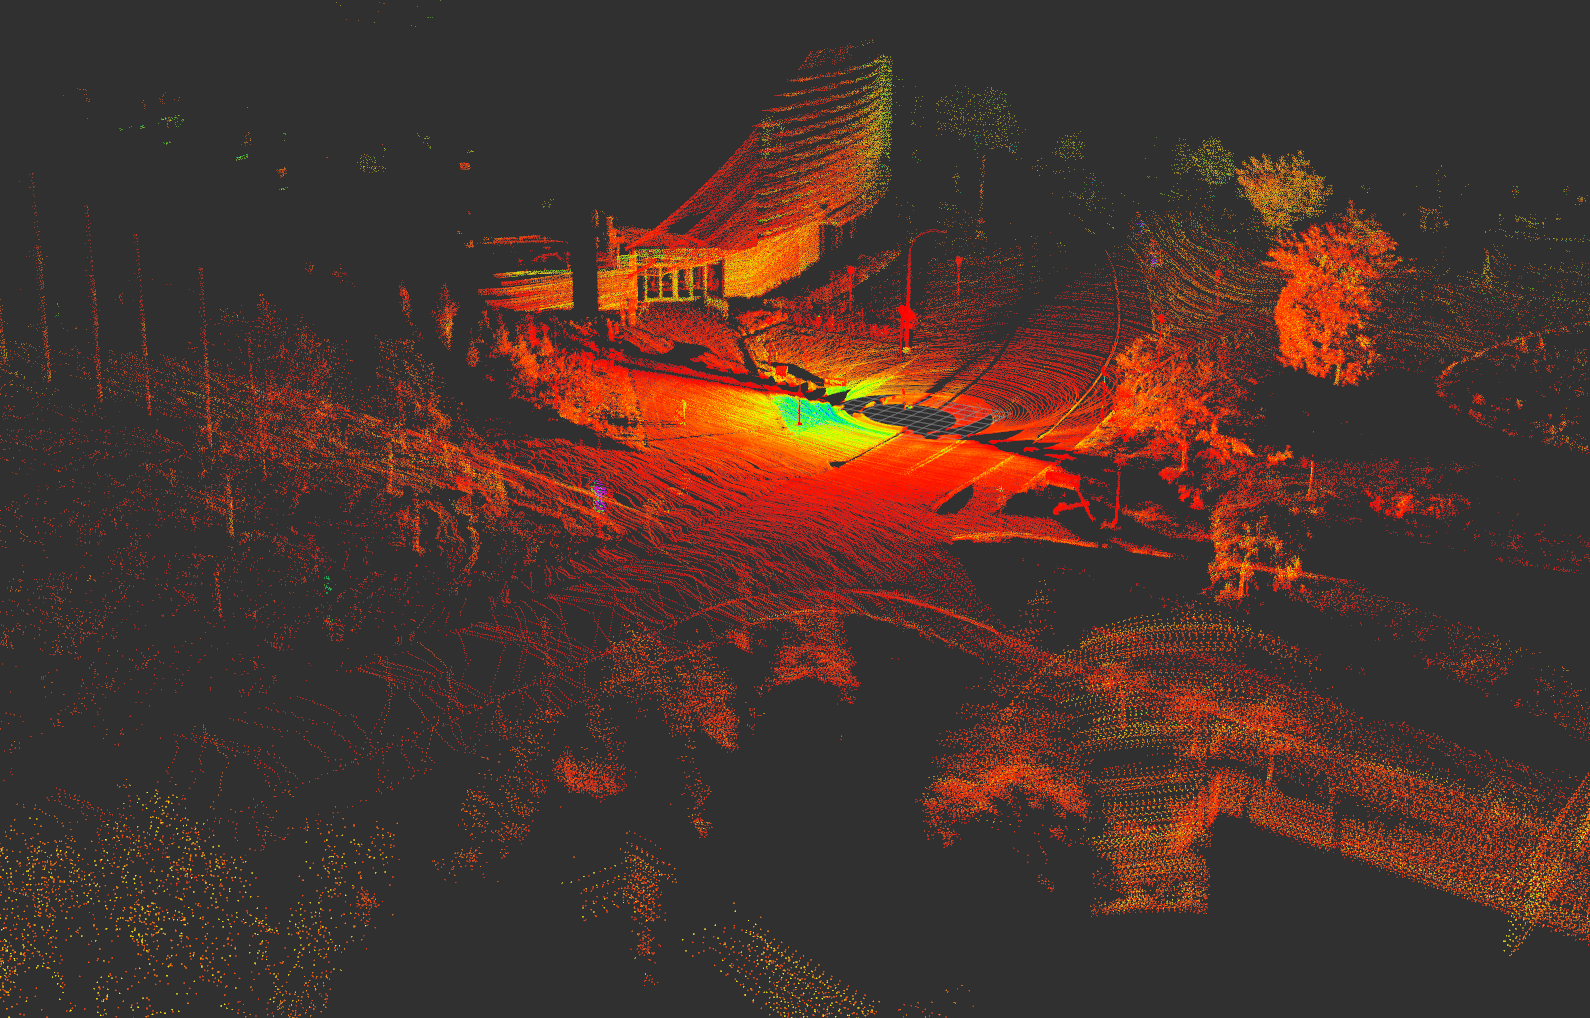
\includegraphics[width=0.45\textwidth]{Chap04MatrixMultiplication/FRBlidarCasseScanBruceHuang.png}}%
\hspace{5pt}%
\subfloat[]{%
	\centering
	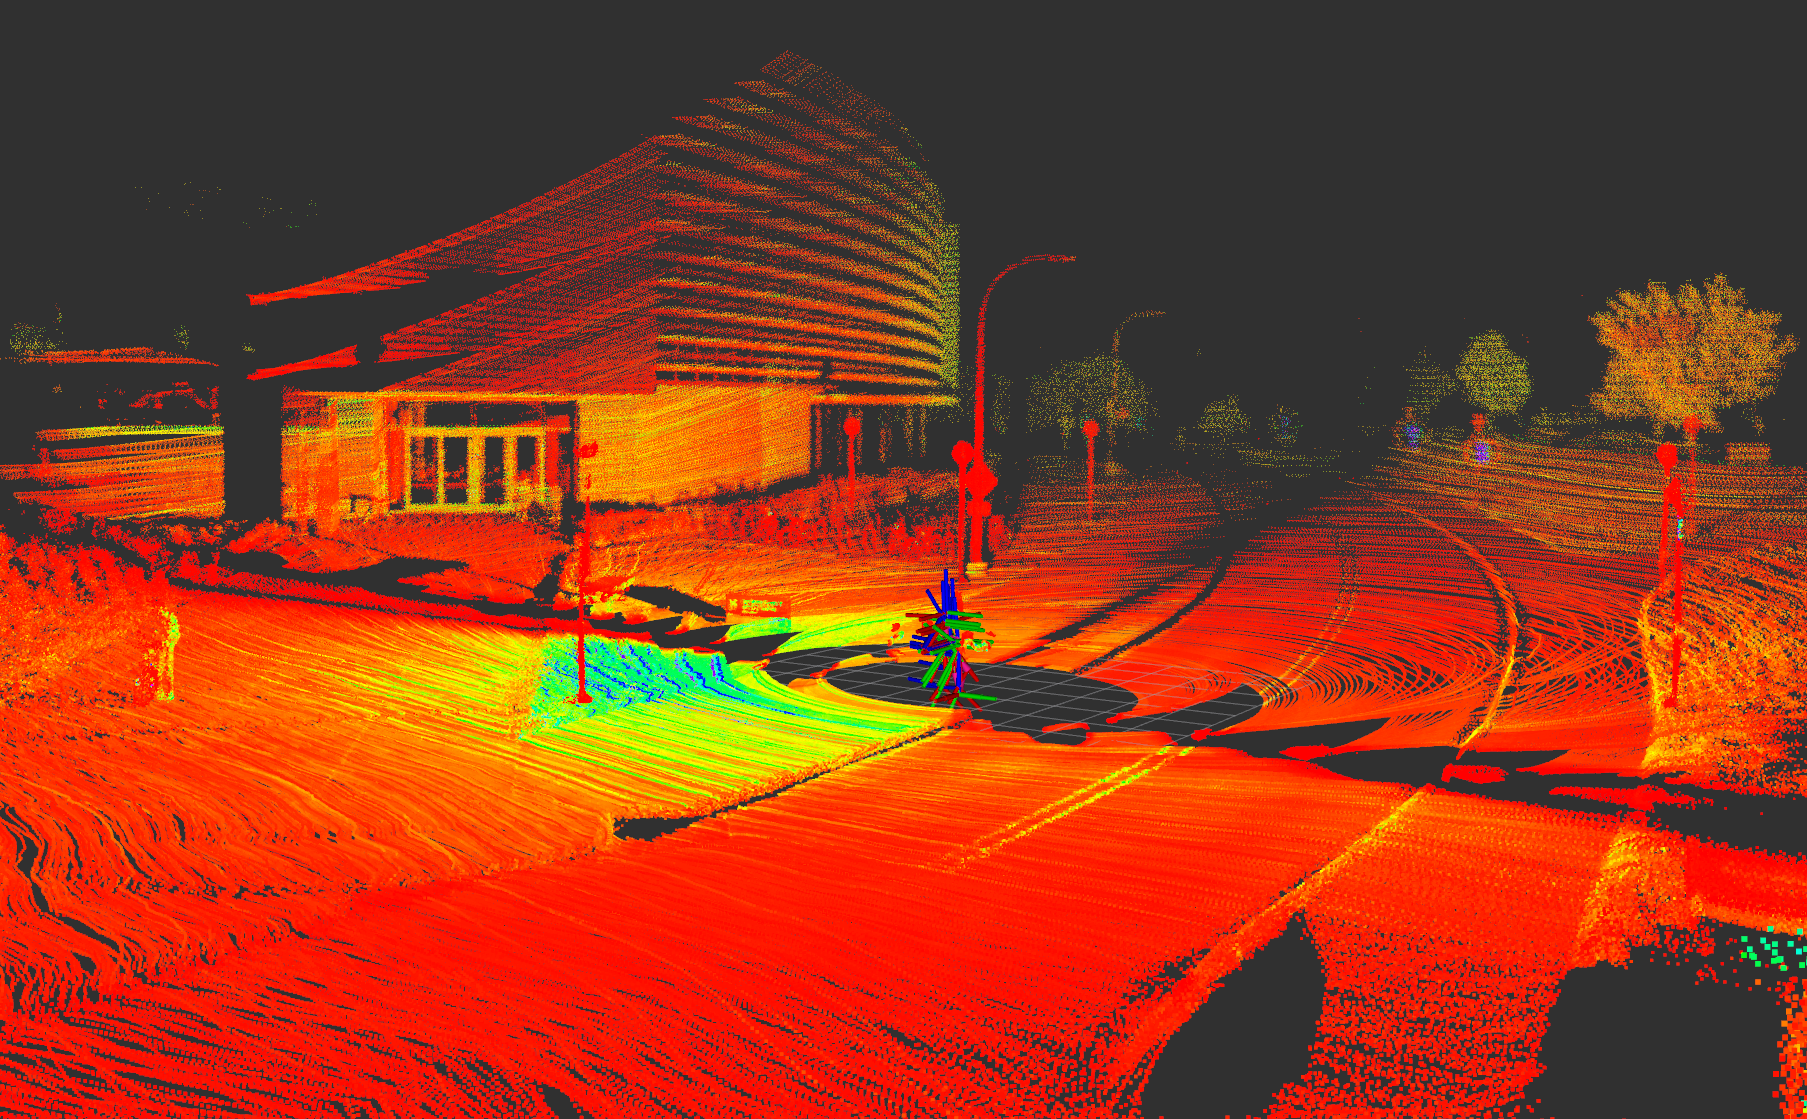
\includegraphics[width=0.465
	\textwidth]{Chap04MatrixMultiplication/FRBlidarCasseScanZoomBruceHuang.png}}%
\caption{Sixty LiDAR images (scans) are combined in this image of the Ford Motor Company Robotics Building. Image courtesy of Bruce Huang. (a) Wide view. (b) Zoom on Cassie's position so you can see the road and the sidewalk. In Project 1, the images are collected while Cassie is walking. You will use matrix-vector multiplication to compensate for Cassie's motion so that the images all appear to be taken from the same position and direction in 3D space. This is called ``image registration''. }
    \label{fig:Chap04MatrixMultiplication/FRBlidarCassieScan}
\end{figure}

\section{(Optional Read): Some Geometric Aspects of Matrix-Vector Multiplication}

Our initial efforts in Computational Linear Algebra focus on the ``algebraic'' part of Linear Algebra, in other words, on equation solving. There are also deep connections with geometry that are used in Robotics. Your Project 1 on Robot Map Building focuses on geometry. We live in a three-dimensional (3D) world and we also find it useful to navigate with two-dimensional (2D) representations of the world, such as Google Maps. \\

How do vectors, matrices, and geometry all come together? Figure~\ref{fig:Chap04MatrixMultiplication/FRBlidarCassieScan} shows a LiDAR image of the Ford Motor Company Robotics Building. The image consists of sixty individual LiDAR images (scans) that have been combined into one single image. The 3D geometry of the building, trees, and even the road passing in front of the building can be clearly seen. That doesn't seem so special, right? We're used to camera images that show even more detail than that! Yes, but while an image today contains millions of pixels, data from a LiDAR are ``sparse'', in the sense that each scan may have only 10,000 points in it, or less than $0.1\%$ of the number of pixels in today's camera images. Each return from one of its lasers gives a 3D point in space, the $(x, y, z)$ coordinates of the point in space off which the laser beam reflected! In addition, the intensity of each laser's return is measured, so we really have a 4-vector $(x, y, z, I)$. While we use the intensity to color the image, we'll ignore it in what follows.

The final image has roughly $60 \times 10,000$ laser returns, that is, points of light, in it, and each point of light in the image is a 3-vector. So, we have roughly $600,000$ 3-vectors in the image. For each of the scans, Cassie's ``head'' was pointing in a different direction. In addition, the body sways a bit. Hence, each of the $10,000$ vectors in an individual scan is being collected from a different position in 3D space, and looking toward a different direction or angle in 3D space, with respect to the other 59 scans. If you were to overlay the 60 images without adjusting for the offsets in position and direction, you would obtain a blurry mess. To see what we mean, just point your cell phone at the night sky sometime with the camera at a long exposure interval; the jittering of your hand will cause a blurry night sky. \\

How to remove the blur? Well, you can declare the position and angle of Cassie in the first scan as a reference and then compensate the vectors in each of the other scans to remove variations in its relative position and angle with respect to the first scan. This compensation process is called ``image registration'' and it can be accomplished by multiplying the $(x, y, z)$ coordinates, which form a 3-vector\footnote{In Project 1, you'll learn that it is better to work with 4-vectors, but the details would be confusing here, so we omit them.}, by an appropriate matrix. \textbf{Bottom line, building a map involves multiplying vectors by matrices, where the matrices somehow encode the relative changes in position and direction of a scan!} \\

Who knew that Cassie had to be a Linear Algebra whiz to build a map! We'll now simplify the problem of imagining how matrices transform 3-vectors by reducing the dimension by one. Moreover, instead of 10,000 2-vectors, we take a single 2-vector $v= \begin{bmatrix} 2.0 \\ 0.5 \end{bmatrix}$ shown in blue in Fig.~\ref{fig:PeakAtMatrixVectorMultiplication} and multiply it by four matrices, 
\begin{enumerate}
\setlength{\itemsep}{.2cm}
\renewcommand{\labelenumi}{(\alph{enumi})}
\item $A_1:=\left[\begin{array}{rr} \cos(\pi/10) & -\sin(\pi/10) \\  \sin(\pi/10) & \cos(\pi/10)\end{array} \right] \implies A_1 v = \left[
\begin{array}{c}
1.7476 \\
1.0936 \\
\end{array}
\right]$
\item $A_2:=\left[\begin{array}{rr} \cos(3 \pi/4) & -\sin(3 \pi/4) \\  \sin(3 \pi/4) & \cos(3 \pi/4)\end{array} \right] \implies A_2 v = \left[
\begin{array}{r}
-1.7678 \\
1.0607 \\
\end{array}
\right]$
\item $A_3:=\left[\begin{array}{rr} 0.5 & 0.0 \\  0.0 & 0.5\end{array} \right] \implies A_3 v = \left[\begin{array}{r}
1.0000 \\
0.2500 \\
\end{array}
\right]$
\item $A_4:=\left[
\begin{array}{rr}
-0.6000 & 0.6000 \\
-0.3360 & -0.0840 \\
\end{array}
\right] \implies A_4 v = \left[
\begin{array}{c}
-0.9000 \\
-0.7140 \\
\end{array}
\right]$
\end{enumerate}
The results are given by the red vectors in Fig.~\ref{fig:PeakAtMatrixVectorMultiplication}. In the context of Cassie and the LiDAR data, Fig.~\ref{fig:PeakAtMatrixVectorMultiplication}-(a) and -(b) are the most relevant as they show a vector being rotated by a fixed angle. Fig.~\ref{fig:PeakAtMatrixVectorMultiplication}-(c) shows a vector being scaled, while Fig.~\ref{fig:PeakAtMatrixVectorMultiplication}-(d) shows a vector that appears to be rotated and scaled. 


\vspace*{.2cm} 
\begin{figure}[hbt!]
\centering
\subfloat[]{%
    \label{fig:Chap4RotateVector}%
	\centering
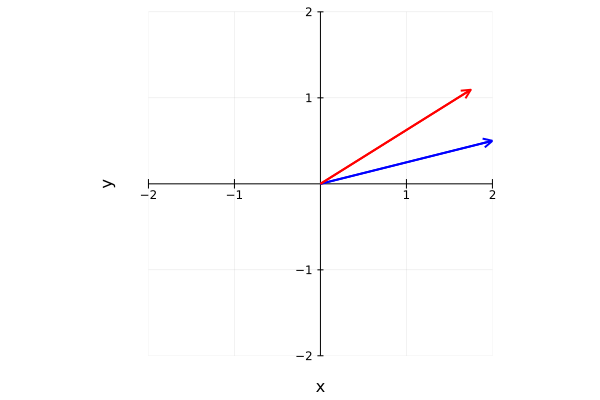
\includegraphics[width=0.4\textwidth]{Chap04MatrixMultiplication/MotivateSmallRotateVector.png}}%
\hspace{5pt}%
\subfloat[]{%
    \label{fig:Chap4ScaleVector}%
	\centering
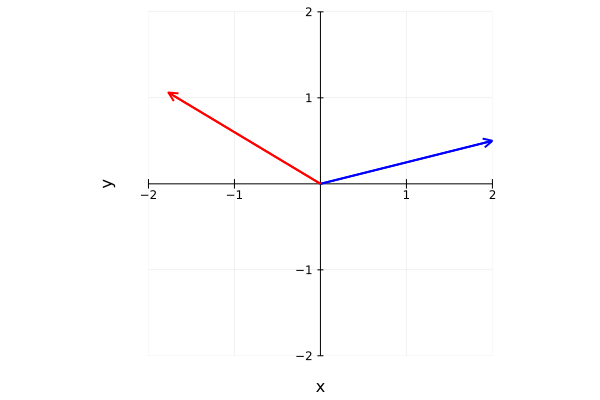
\includegraphics[width=0.42\columnwidth]{Chap04MatrixMultiplication/MotivateRotateVector.png}}%
\hspace{5pt}%
\subfloat[]{%
    \label{fig:Chap4ScaleVectorB}%
	\centering
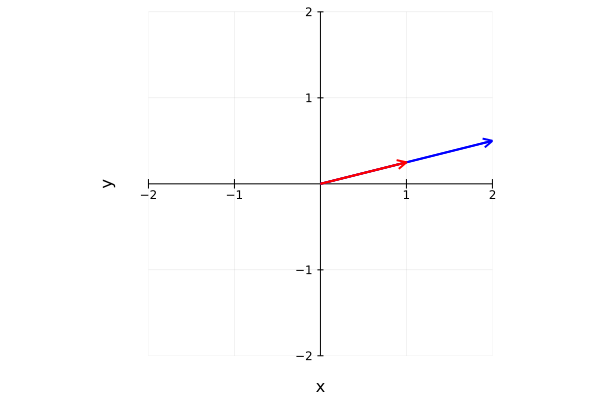
\includegraphics[width=0.42\columnwidth]{Chap04MatrixMultiplication/MotivateScaleVector.png}}%
\hspace{5pt}%
\subfloat[]{%
    \label{fig:Chap4ScaleVectorC}%
	\centering
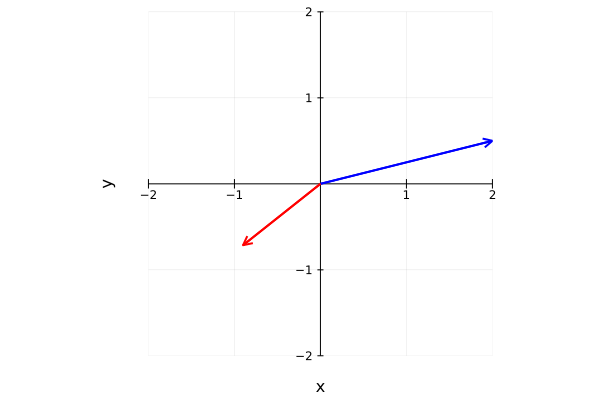
\includegraphics[width=0.42\columnwidth]{Chap04MatrixMultiplication/MotivateGeneralVector.png}}%
\caption{The vector $v$ is in blue while the transformed vector, $A v$, is shown in red. (a) The matrix rotates the blue vector clockwise by an angle of $\pi/10$ or 18$^o$. (b) The matrix rotates the blue vector clockwise by an angle of $3 \pi/4$ or 135$^o$. (c) The matrix scales the blue vector by 0.5. And (d), the matrix acts on the blue vector in a general fashion that we will be able to ``decode'' when we study eigenvalues and eigenvectors in Chapter 10.}
\label{fig:PeakAtMatrixVectorMultiplication}
\end{figure}
% (c) The matrix scales the $x$-component of the blue vector by 0.5 and its $y$-component by 1.0. 

\section{Looking Ahead}

Once again, our first major goal in the course is to solve very large sets of linear equations, say more than 100 variables. In the previous chapter, we saw how to solve problems with triangular structure. In this Chapter, we learned how to multiply two matrices.\\

Let's use our knowledge and see what happens when we multiply a lower triangular matrix times an upper triangular matrix. We define two matrices by $L$ and $U$ for lower and upper triangular, respectively, 
$$L=\left[\begin{array}{rrr} 1 & 0 & 0\\
-2 & 1 & 0 \\ 3 & -2 & 1  \end{array}\right]~~\text{and}~~U=\left[\begin{array}{rrr} 
    3 & 3 & 2\\
0 & 6 & 1 \\ 
0 & 0 & -3  \end{array}\right] \implies L\cdot U = \left[ \begin{array}{rrr}
     3   &  3  &   2 \\
    -6   &  0  &  -3 \\
     9  &  -3    &  1 \\
\end{array} \right] =:A. $$
Hence the product of a lower triangular matrix and an upper triangular matrix seems to be a ``general matrix'' $A$, meaning it has no particular structure. \\

\textbf{Question:} Is it possible to go backwards? That is, starting with a general matrix $A$, is it possible to write it as the product of a lower triangular matrix and an upper triangular matrix? And if it is possible, is it useful? What's the trick?\\

\textbf{Answers:} Yes. Very! Our alternative way of doing matrix multiplication.\\
